\begin{section}{Methodology and Data }

\begin{subsection}{Methodology }

To answer our research question, our specifications need to allow for the possibility of trade creation and trade diversion. \autoref{tab_2} gives an overview about the potential magnitudes involved. 

\begin{table}[H]
\centering
\begin{tabular}{lccc} 
\hline
                                             & \textbf{Intra-bloc trade}                                                         & \multicolumn{2}{c}{\begin{tabular}[c]{@{}c@{}}\textbf{Extra-bloc trade}\\ \end{tabular}}                                                                                 \\ 
\cline{2-4}
                                             & \begin{tabular}[c]{@{}c@{}}\textbf{Trade between }\\\textbf{members}\end{tabular} & \begin{tabular}[c]{@{}c@{}}\textbf{Export to }\\\textbf{non-members}\end{tabular} & \begin{tabular}[c]{@{}c@{}}\textbf{Import from }\\\textbf{non-members}\end{tabular}  \\ 
\hline
\multicolumn{1}{c}{\textbf{Trade creation}}  & $\gamma_1 > 0$                                                                    & $\delta_1 > 0$                                                                    & $\delta_2 > 0$                                                                       \\
\multicolumn{1}{c}{\textbf{Trade diversion}} & $\gamma_1 < 0$                                                                    & $\delta_1 < 0$                                                                    & $\delta_2 < 0$                                                                       \\
\hline
\end{tabular}
\caption{\small{Potential Magnitudes: Trade Creation and Trade Diversion Effects as in Specification 1.}}
\label{tab_2}
\end{table}

Since our aim is to compare the effects of ACFTA on bilateral trade flows within ACFTA to ACFTA-sourced imports from third countries and ACFTA-directed exports from third countries as in \autoref{tab_2}, we make use of three corresponding dummy variables:

$ACFTA$ estimates the impact of the commencement of the agreement on ASEAN-China trade flows. Throughout all specifications, $ACFTA$ takes the value one when countries $i$ and $j$ belong to ACFTA in year $t$ and zero if otherwise. A positive (negative) coefficient $\gamma_1$ represents trade creation (diversion), depending on whether intra-bloc trade is higher (lower) than the normal trade levels due to the trade agreement. 

$ACFTAexport$ takes a value of one if exporter country $i$ belongs to the ACFTA in year $t$ and destination country $j$ does not belong to the ACFTA countries and zero otherwise. A statistically significant and positive $\delta_1$ coefficient can be interpreted as an export creation effect. It implies that regional trade integration leads to export diversion from ACFTA member countries to non ACFTA countries. However, a negative $\delta_1$ coefficient signifies an export reduction between member countries and non-member countries, known as the export diversion effect (\cite{carrere_2006}). 

$ACFTAimport$ takes a value of one if exporter $i$ is a non-member country of ACFTA in year $t$ and destination country $j$ belongs to the ACFTA member countries and zero otherwise. Essentially, a statistically significant and positive $\delta_2$ coefficient captures an import creation effect, showing the expansion of imports from the non-member countries to member countries. Contrarily, a negative $\delta_2$ coefficient indicates the import diversion effect, a decrease in imports from non-member- to member countries (\cite{carrere_2006}).

It is this triad of dummy variables that enables us to obtain evidence on the so-called Viner ambiguity in the context of the ACFTA (see \autoref{tab_2}). Our study is to be viewed as adding robustness to \cite{smz2014} and \cite{wla_2021}.

In addition, we control for trade effects that countries sharing another FTA with ACFTA countries have. As \autoref{fig_3} shows, conceptually, these third-country effects are made up by both the trade flows between single ACFTA member countries and their respective partner countries (“Own-ACFTA effect”) as well as countries neither belonging to the set of either ACFTA or ACFTA partner countries ("Cross-ACFTA effect”). In our specifications, their combined effect is captured by the $otherRTA$ dummy, similar to the concept of interdependence of RTAs introduced in \cite{bbm2014}.


\begin{figure}[H]
	\centering
	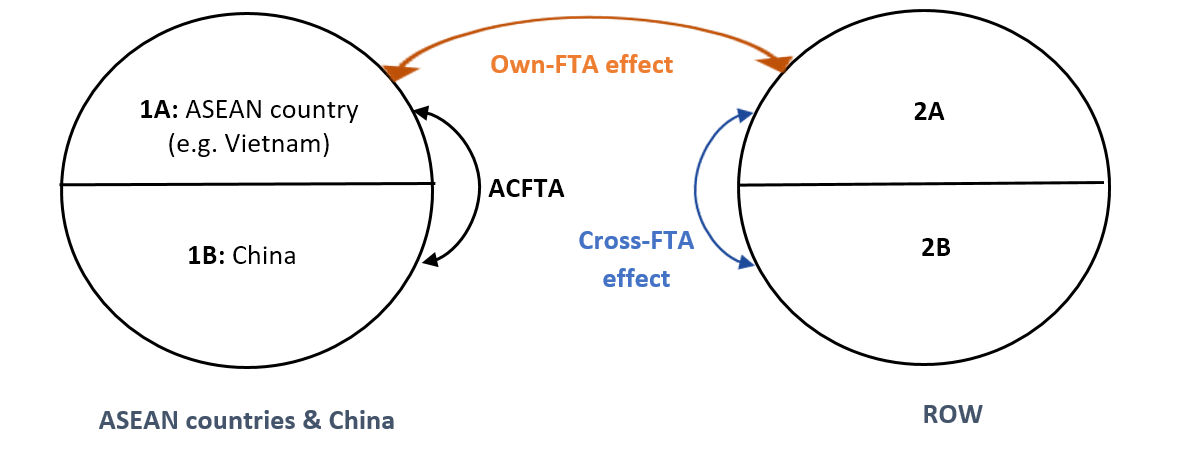
\includegraphics[width=\textwidth]{figure_3.png}
	\caption{\small{Trade Creation and Trade Diversion: Own-FTA effects and Cross-FTA effects.}}
	\label{fig_3}
\end{figure}

Our ex-post assessment of the trade effects of ACFTA starts with a naïve regression specification. Stepwise, we include additional modifications. Each modification introduces a new feature to the initial specification, aiming at correctly identified estimates of the four ACFTA effects which we focus on.


\subsubsection*{Specification 1: OLS estimation ignoring multilateral resistance terms}

We first do an OLS estimation of the empirical specification that includes standard gravity variables with panel data with 4-year intervals\footnote{Interval panel data should be employed in order to allow for adjustment in bilateral trade flows in response to trade policy or other changes in trade costs (\cite{ypl_2016})}:

\begin{multline}\label{eq_4}
lnTrade_{ijt} = \alpha_0 + \beta_1 lnY_{it} + \beta_2 lnY_{jt} + \beta_3 lnPop_{it} + \beta_4 lnPop_{jt}  + \beta_5 lnDist_{ij} + \beta_6 Lang_{ij} + \beta_7 Contig_{ij} + \\
\gamma_1 ACFTA_{ijt} + \gamma_2 otherRTA_{ijt} + \\ 
\delta_1 ACFTAexport_{ijt} + \delta_2 ACFTAimport_{ijt} + \epsilon_{ijt}
\end{multline}

In this basic gravity model, we make aggregate total bilateral trade flows $lnTrade$ from to country $j$ to country $i$ dependent on Gross Domestic Product ($lnY$), population ($lnPop$) and distance ($lnDist$). Moreover, we include the binary dummies common border ($Contig$) and language ($Lang$). 


\subsubsection*{Specification 2: OLS estimation controlling for multilateral resistance terms with fixed effects}
Specification \ref{eq_4} is modified to account for the multilateral resistances with an appropriate set of exporter-time and importer-time fixed effects to control for the unobservable multilateral resistances (\cite{avw2003}).

\begin{multline}\label{eq_5}
\ln{Trade_{ijt}} = \mu_{it} + \phi_{jt} + \beta_5 \ln{Dist_{ij}} + \beta_6 Lang_{ij} + \beta_7 Contig_{ij} + \\ \gamma_1 ACFTA_{ijt} + \gamma_2 otherRTA_{ijt} + \\
\delta_1 ACFTAexport_{ijt} + \delta_2 ACFTAimport_{ijt} + \epsilon_{ijt}
\end{multline}

$\mu_{it}$ denotes the vector of exporter-time fixed effects, which accounts for the outward multilateral resistances. Similarly, the vector $\phi_{jt}$ denotes the set of importer-time fixed effects to capture the inward multilateral resistances. No constant term is included in the presence of the fixed effects. By definition, both exporter-time and importer-time fixed effects will absorb, respectively, the values of exporter output and importer expenditure, as well as all other observable and unobservable exporter- and importer-specific characteristics that may influence bilateral trade.


\subsubsection*{Specification 3: PPML estimation controlling for multilateral resistance terms with fixed effects}

Specification \ref{eq_5} is re-formulated in multiplicative form and re-estimated by applying the PPML estimator to the same sample.

\begin{multline}\label{eq_6}
Trade_{ijt} = exp \Big(\mu_{it} + \phi_{jt} + \beta_5 lnDist_{ij} + \beta_6 Lang_{ij} + \beta_7 Contig_{ij} \\ 
+ \gamma_1 ACFTA_{ijt} + \gamma_2 otherRTA_{ijt} + \\
\delta_1 ACFTAexport_{ijt} + \delta_2 ACFTAimport_{ijt}\Big) \epsilon_{ijt}
\end{multline}

\bigskip
Applying the PPML estimator to the gravity model is justified on various grounds. First, the PPML estimator expressed in a multiplicative form, accounts for heteroscedasticity, which often plagues trade data (\cite{silva2006log}). Second, for the same reason, the PPML estimator is able to take advantage of the information contained in the zero trade flows. Third, the additive property of the PPML estimator ensures that the gravity fixed effects are identical to their corresponding structural terms (\cite{fally2015}).

\subsubsection*{Specification 4: Addressing potential endogeneity of FTAs}

Without further ado, trade effects from the formation of ACFTA could have lied fault to a chicken egg problem of reverse causality. Following \cite{ypl_2016}, specification \ref{eq_6} is modified to include country-pair fixed effects $\pi_{ij}$ in addition to the importer-time and exporter-time fixed effects $\mu_{it}$ and $\phi_{jt}$.

\begin{multline}\label{eq_7}
Trade_{ijt} = exp \Big(\mu_{it} + \phi_{jt} + \pi_{ij} + \\ 
\gamma_1 ACFTA_{ijt} + \gamma_2 otherRTA_{ijt} +  \\
\delta_1 ACFTAexport_{ijt} + \delta_2 ACFTAimport_{ijt}\Big) \epsilon_{ijt}
\end{multline}

Our rationale stems from \cite{bb_2007} who warn of omitted variable bias and simultaneity bias. 
To illustrate a potential source of omitted variable bias, let us suppose two countries with extensive domestic regulations inhibiting trade. Then, once a large expected welfare gain from trade creation via the FTA in sight, the likelihood of the countries selecting into the FTA could have been especially high. 
Simultaneity bias can be illustrated as follows: suppose two countries trade more or less than the gravity-equation-suggested “natural” level. This could be due to an already extensive trading relationship. Contrarily, one can imagine political pressures to avoid trade liberalisation. In both cases, the problem is that the decision to form an FTA is likely influenced by trade relative to the “natural” level. In contrast, recent changes in trade levels are unlikely to influence FTA formations. Hence, looking at recent changes in trade levels between country pairs allows control for the “natural” level of trade. The idea is that unobserved time invariant heterogeneity, hidden in the “natural” level of trade, simultaneously influences the presence of a FTA and the volume of trade. Using panel data we can control for this unobserved time invariant heterogeneity. Exploiting cross-sectional unit variation over time, we can be reassured about identification. 


\begin{subsubsection}{Our Hypotheses}
Our literature at hand, we expect overall trade creation due to ACFTA. We expect this both within the ACFTA bloc and between the ACFTA bloc and its partners. Hence, our first hypothesis is that $\gamma_1$, $\delta_1$ and $\delta_2$ are positive in sign for ACFTA and its third export and import partners (see \autoref{tab_2}).

Our second hypothesis is placed within the context of trade diversion. \cite{dyz_2014} find that an outside FTA with another country reduces trade volume, especially on the importer-side. The magnitude of the importer-side estimate is economically large and statistically significant. On average, countries that joined FTAs during the sample period imported 57\% less from non-FTA partners. As opposed to \cite{dyz_2014}, we expect the coefficient of the $otherRTA$ dummy to be positive for ACFTA, reflecting trade creation from both an "Own-ACFTA" as well as a "Cross-ACFTA" effect (see \autoref{fig_3}).
\end{subsubsection}


\end{subsection}



\begin{subsection}{Data}

This study uses unbalanced panel data of bilateral trade flows, GDP, population, distance, geographical, cultural and historical information and a few other group-specific measures from \cite{cepii-data_2022}.

The gravity models include 252 countries covering the period 1995-2019 (24 years). The source of information for aggregated (country-level) bilateral trade flows is BACI trade data downloaded from \cite{cepii-data_2022}. The reason for choosing BACI data for the dependent variable is twofold: first, BACI data are cleaned to exclude re-exports. Second, BACI data reconcile reporting differences among countries. Therefore, BACI data provide a more complete and coherent set of trade flows than for example UN Comtrade import data. We however stick to UN Comtrade import data to replace missing values of BACI trade flows. Again, there are two reasons. First, BACI trade flows stem from the UN Comtrade database. Second, import data is considered more reliable because imports are monitored much more closely than exports by customs administrations, see \cite{ypl_2016}.

Data on RTAs is constructed based on the World Trade Organization Regional Trade Arrangements Database, see \cite{wto-data_2022}. 

Please, find the data for replication \href{https://github.com/gerodasbach/data_repository_RIA_report.git}{here}.\footnote{Due to the large size of the original data set, it is not part of the github repository. We offer to transfer it and suggest you to insert it manually into your \textit{./input} folder. Please contact us per \href{mailto:gero.dasbach@gmail.com}{e-mail}.}

\end{subsection}
\end{section}